\section{Visual Design}

\subsection{Event}
An event is represented as a line of text -- \emph{label} -- summarizing its content, and a glyph indicating its temporal information. For a time-point event, a \emph{circle} is shown at the left of the label. For an interval event, a \emph{bar} is shown at the top of the label. When two interval events overlap, their time bars are displayed with half transparency to make the intersection visible. To accommodate a large number of events, labels have three possible levels of detail: 
\begin{enumerate}
	\item \textbf{Complete}. The entire label is shown.
	\item \textbf{Trimmed}. Only the first few words are shown and ended with three dots (\dots) to indicate that the visible label is incomplete.
	\item \textbf{Aggregated}. Events are grouped and labeled with the total number of them. A colored border is added to the label to make the aggregate more noticeable. The time bar of an aggregate spans the starting time of its earliest event and the finishing time of its latest event.
\end{enumerate}	

Figure~\ref{fig:event-representation} shows examples these different visual representation of events.

\begin{figure}[!htb]
\centering
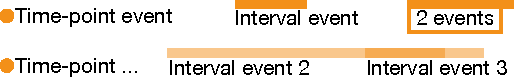
\includegraphics[width=.8\columnwidth]{figure2}\caption{Visual representations of events. Top row, left to right: a complete time-point event, a trimmed time-point event, and a aggregate of 10 events. Bottom row, left to right: an interval event, and two overlapping interval events.}
\label{fig:event-representation}
\end{figure}

\subsection{Set}
\subsubsection{Design Overview}
Similar to SchemaLine (Section~\ref{sub:schema}), TimeSets also applies the same Gestalt principles in its design: \emph{connectedness} and \emph{proximity}. Events belonging to the same set are located close together, and the background of an entire set is colored to make its events visually connected. Spatial grouping needs to be achieved through vertical positioning because the horizontal position of each event is already determined by its temporal information. Sets are stacked vertically, and each set is further divided into a maximum of three \emph{layers}: the top and the bottom layer for events shared with the set above and below respectively (if they exist), and the middle layer for other events in the set. Figure~\ref{fig:layering} shows an example of a layering for three sets.

\begin{figure}[!htb]
\centering
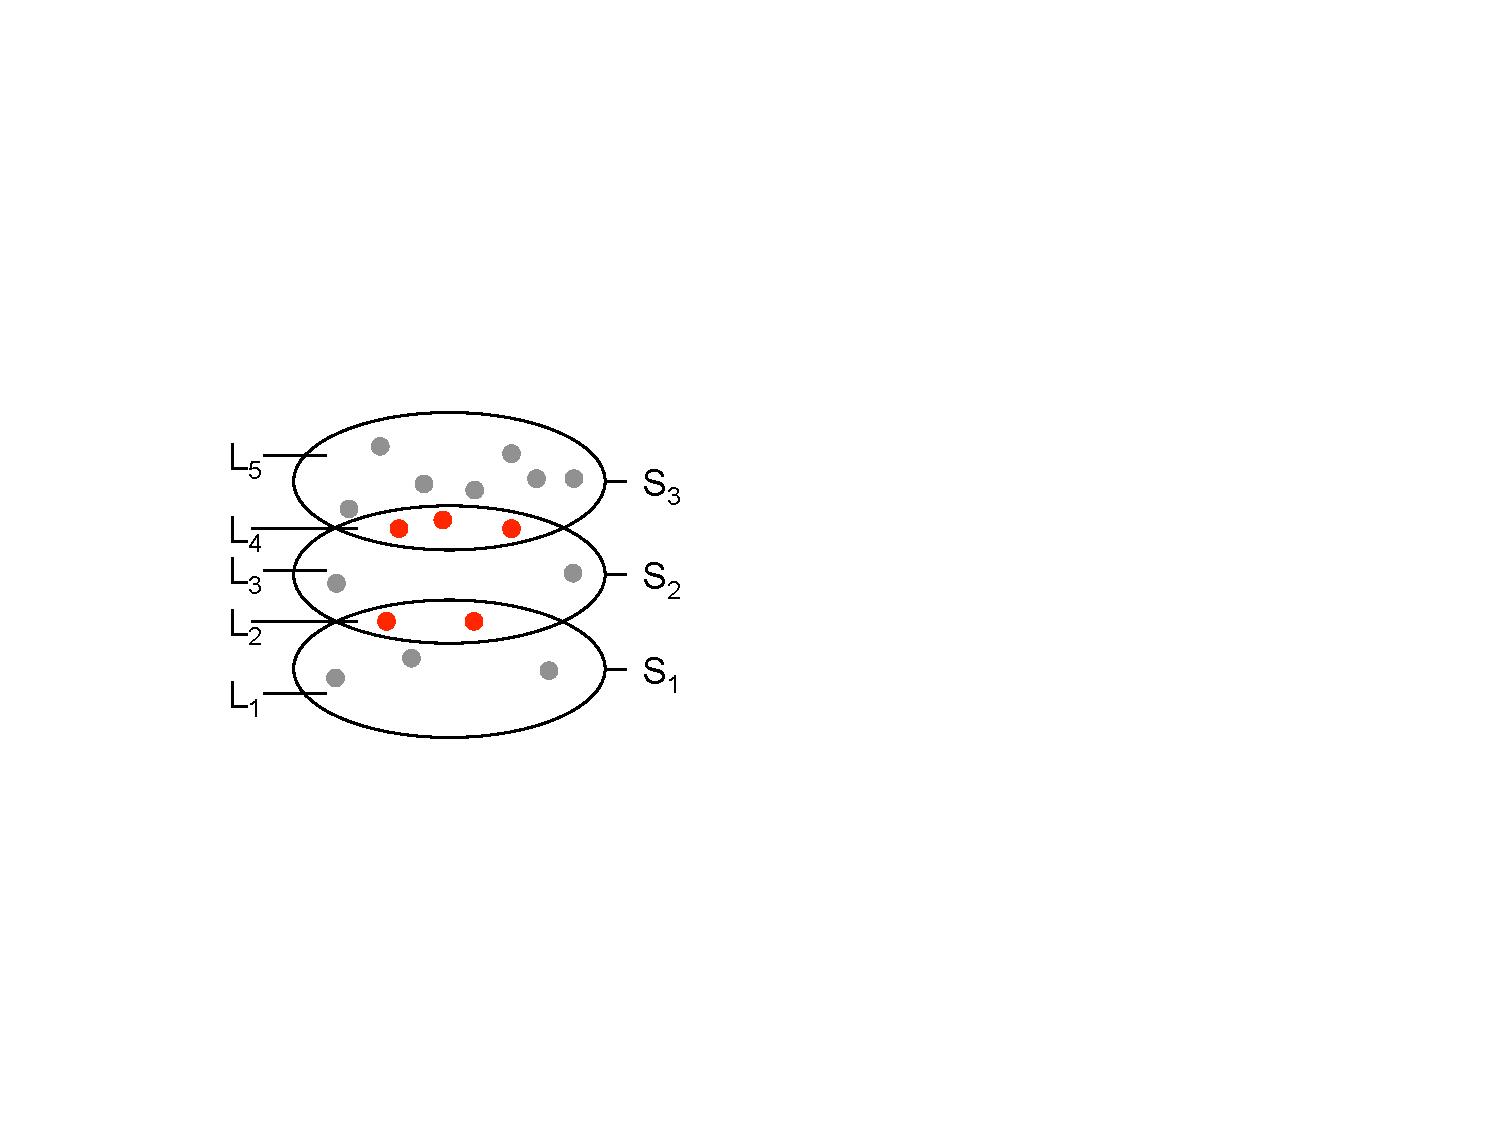
\includegraphics[width=.5\columnwidth]{figure3}
\caption{Layering for three sets $S_1$, $S_2$, and $S_3$. $L_2$ includes events shared by $S_1$ and $S_2$, and $L_4$ includes events shared by $S_2$ and $S_3$. Shared events are shown in red. $S_2$ consists of events in three layers $L_2$, $L_3$, and $L_4$.}
\label{fig:layering}
\end{figure}

Shared events between two non-neighboring sets can reside in one set and connect to the other set using visual links such as curves~\cite{Alper2011} or areas~\cite{Meulemans2013}. Figure~\ref{fig:layering-1} shows an approach to connect shared events (red squares) using straight edges and link them to the orange set to indicate that they also belong to that set. An alternative approach is to duplicate shared events in both sets. In Figure~\ref{fig:layering-2}, red squares are duplicated in both the green and orange sets. Duplication consumes more display space and could make viewers confuse when seeing same events multiple times. However, it ensures all events of the same set being located close together, which makes the visualization compact. Also, a study by Henry Riche and Dwyer~\cite{Riche2010} shows that complex set-intersection shapes reduce readability compared to item duplication. Aiming for a clear visualization, which is crucial for interactive set construction, we decide to duplicate events that belong to non-neighboring sets. Confused duplication and scalability will be addressed later using interaction and layout algorithm respectively.

\begin{figure}[!htb]
	\centering
	\subcaptionbox{Shared events are located in the green set, and linked to the orange set.\label{fig:layering-1}}[.47\columnwidth]
	{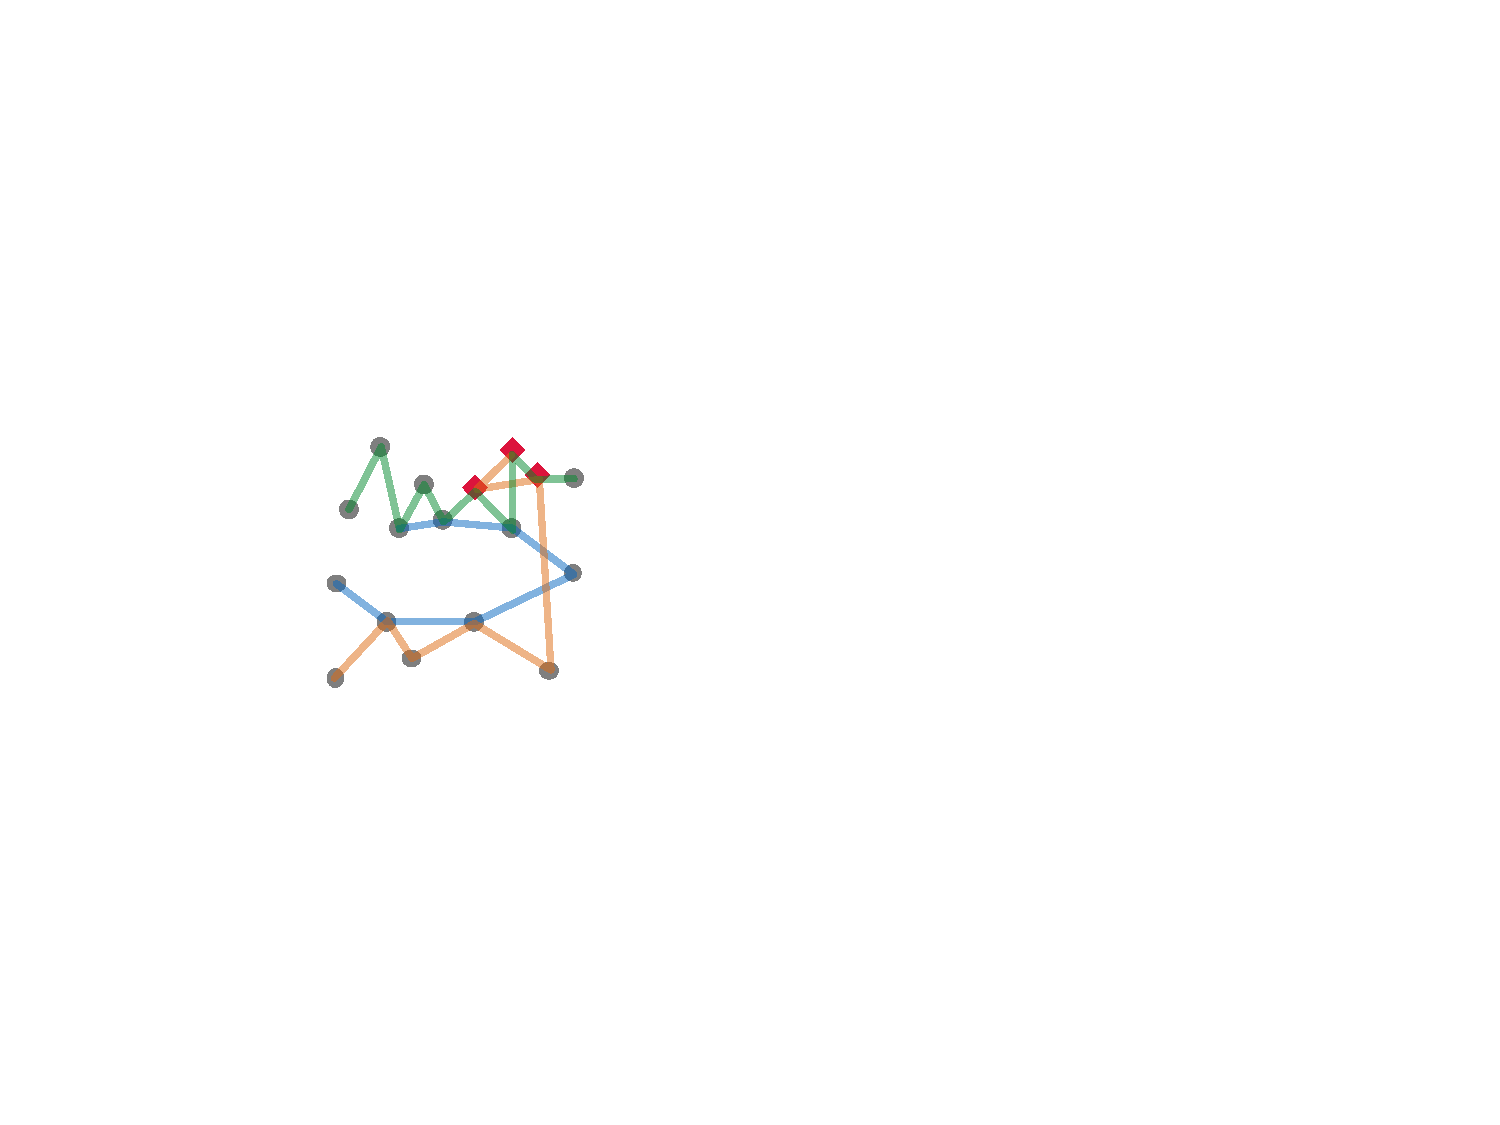
\includegraphics[width=.35\columnwidth]{figure4a}}
	\hfill	
	\subcaptionbox{Shared events are duplicated in both green and orange sets.\label{fig:layering-2}}[.47\columnwidth]
	{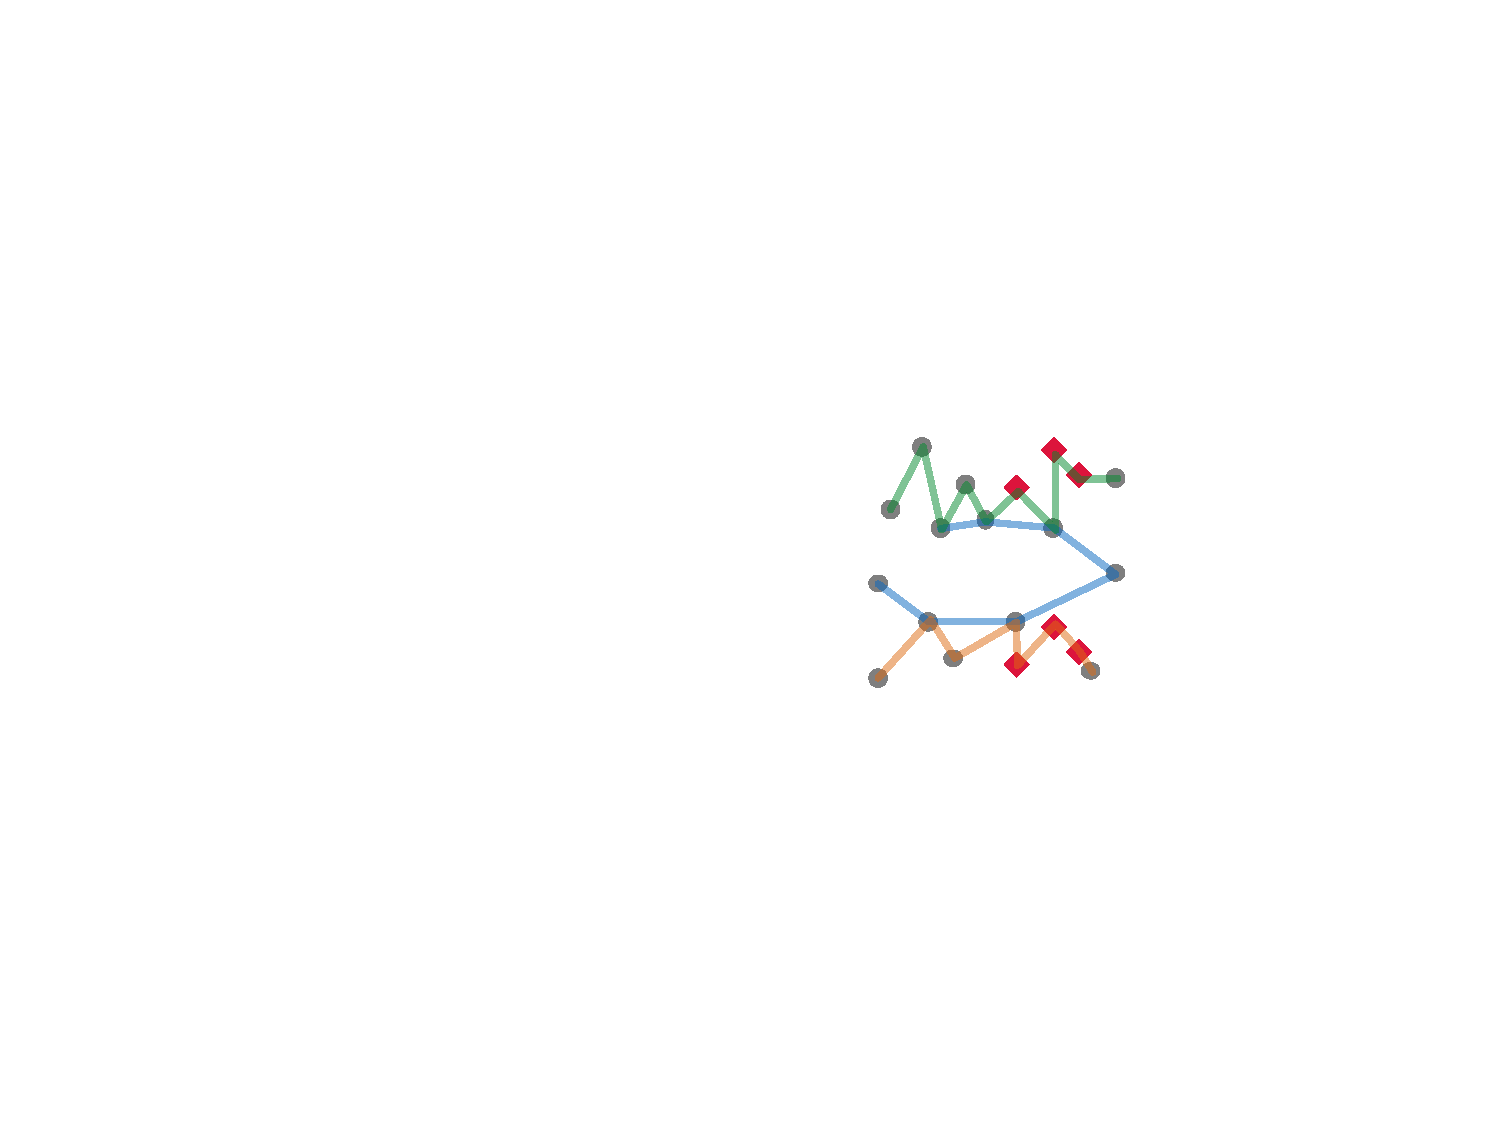
\includegraphics[width=.35\columnwidth]{figure4b}}
	\caption{Visualizations of shared events between two non-neighboring sets (red squares).}
	\label{fig:layering-compare}
\end{figure}

In subsequent sections, we discuss the detail of the set visualization algorithm, which consists of two main steps: generating set shapes, and then coloring them.

\subsubsection{Shape Generation}
\label{sub:shapesgeneration}
This algorithm takes as input a list of bounding-boxes of all events in a set, and generates a closed-curve containing all these boxes. The sizes and positions of the bounding boxes are decided by the layout algorithm described in the next section. A rectilinear shape can be generated using a scan-line algorithm~\cite{Foley1997}, as shown in Figure~\ref{fig:shape1}. The number of bends along the border is often used to assess the aesthetics and legibility of visualizations~\cite{Tanahashi2012}. Even though the generated shape provides the minimal \textit{data-ink} ratio~\cite{Tufte1983}, a large number of line bends may reduce its legibility. 

\begin{figure}[!htb]
	\centering
	\subcaptionbox{The original rectilinear shape generated by a scan-line algorithm.\label{fig:shape1}} 
	{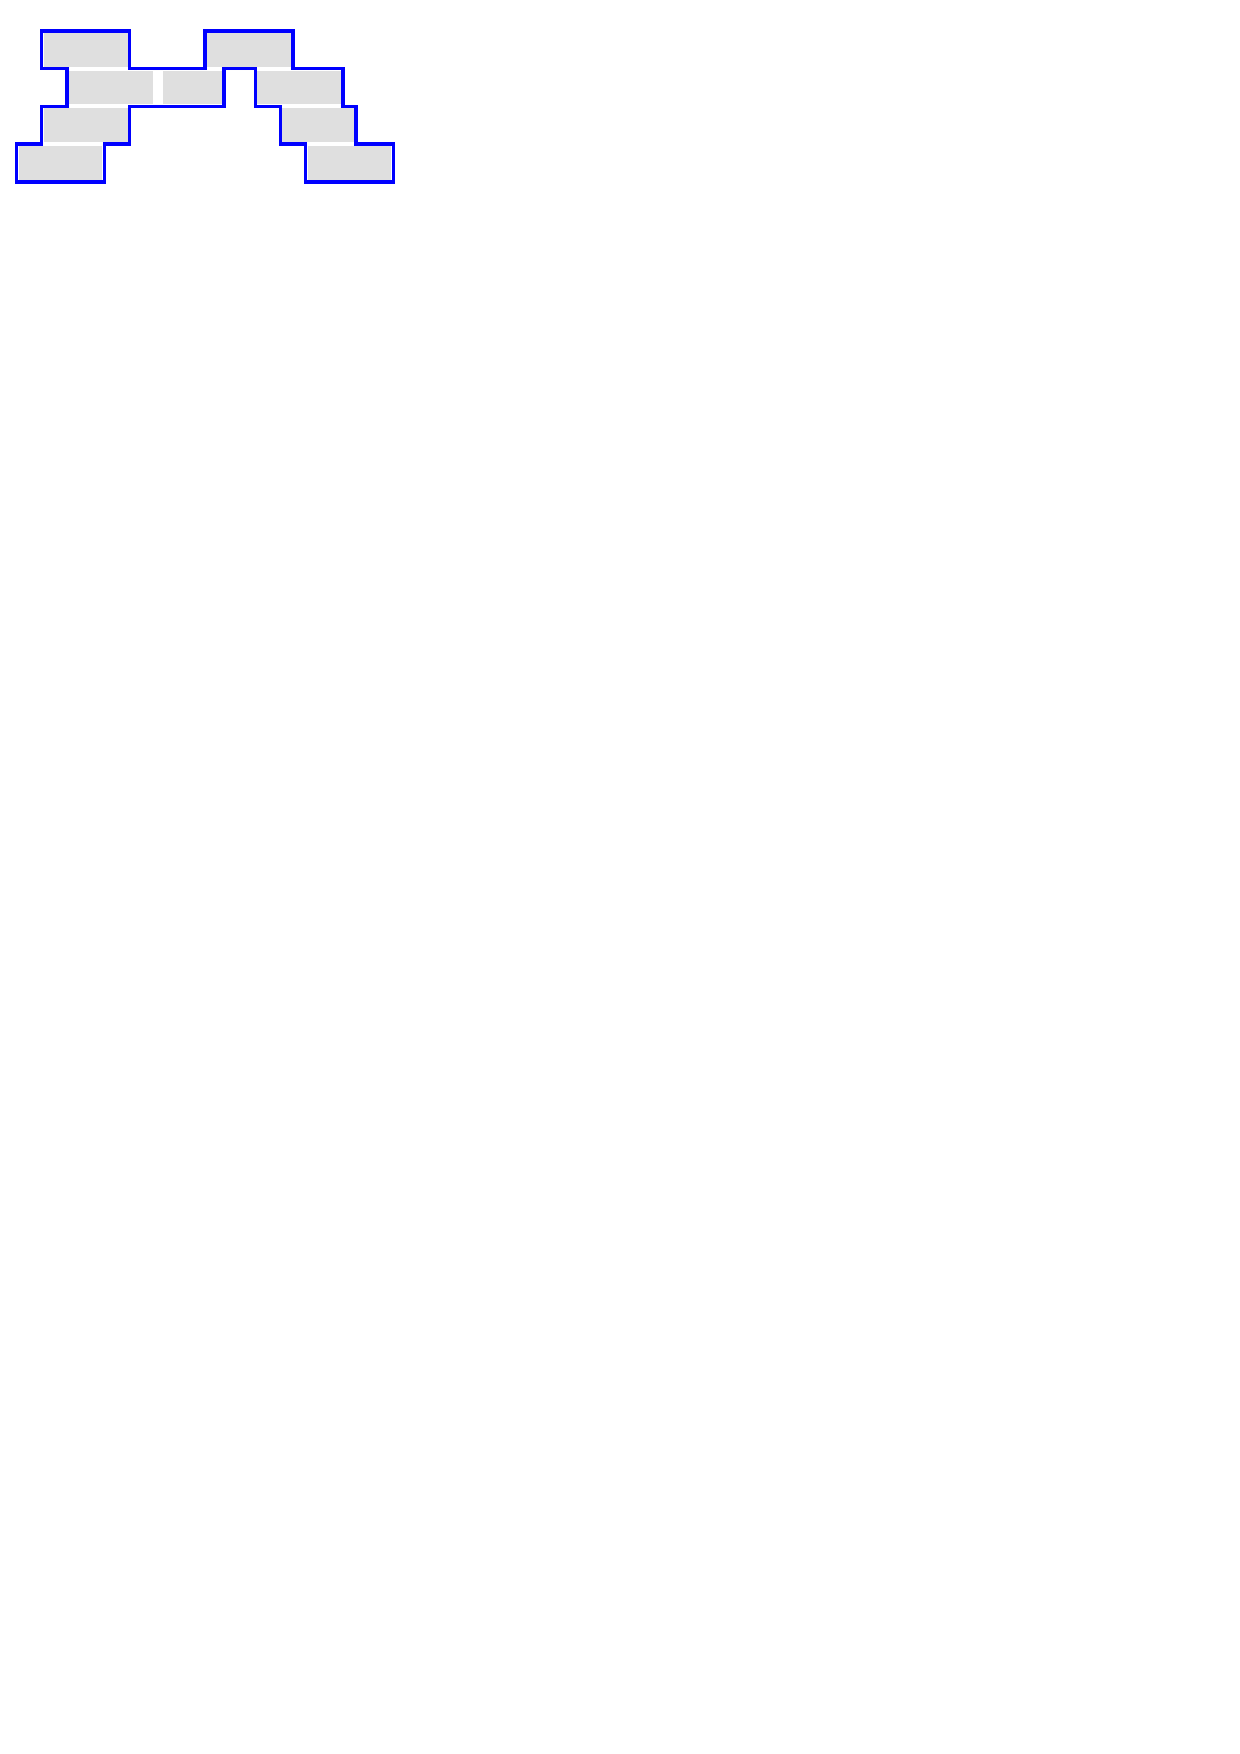
\includegraphics[width=.47\columnwidth]{figure5a}}
	\hfill
	\subcaptionbox{The simplified shape by flattening and removing jags (red eclipse).\label{fig:shape2}}
	{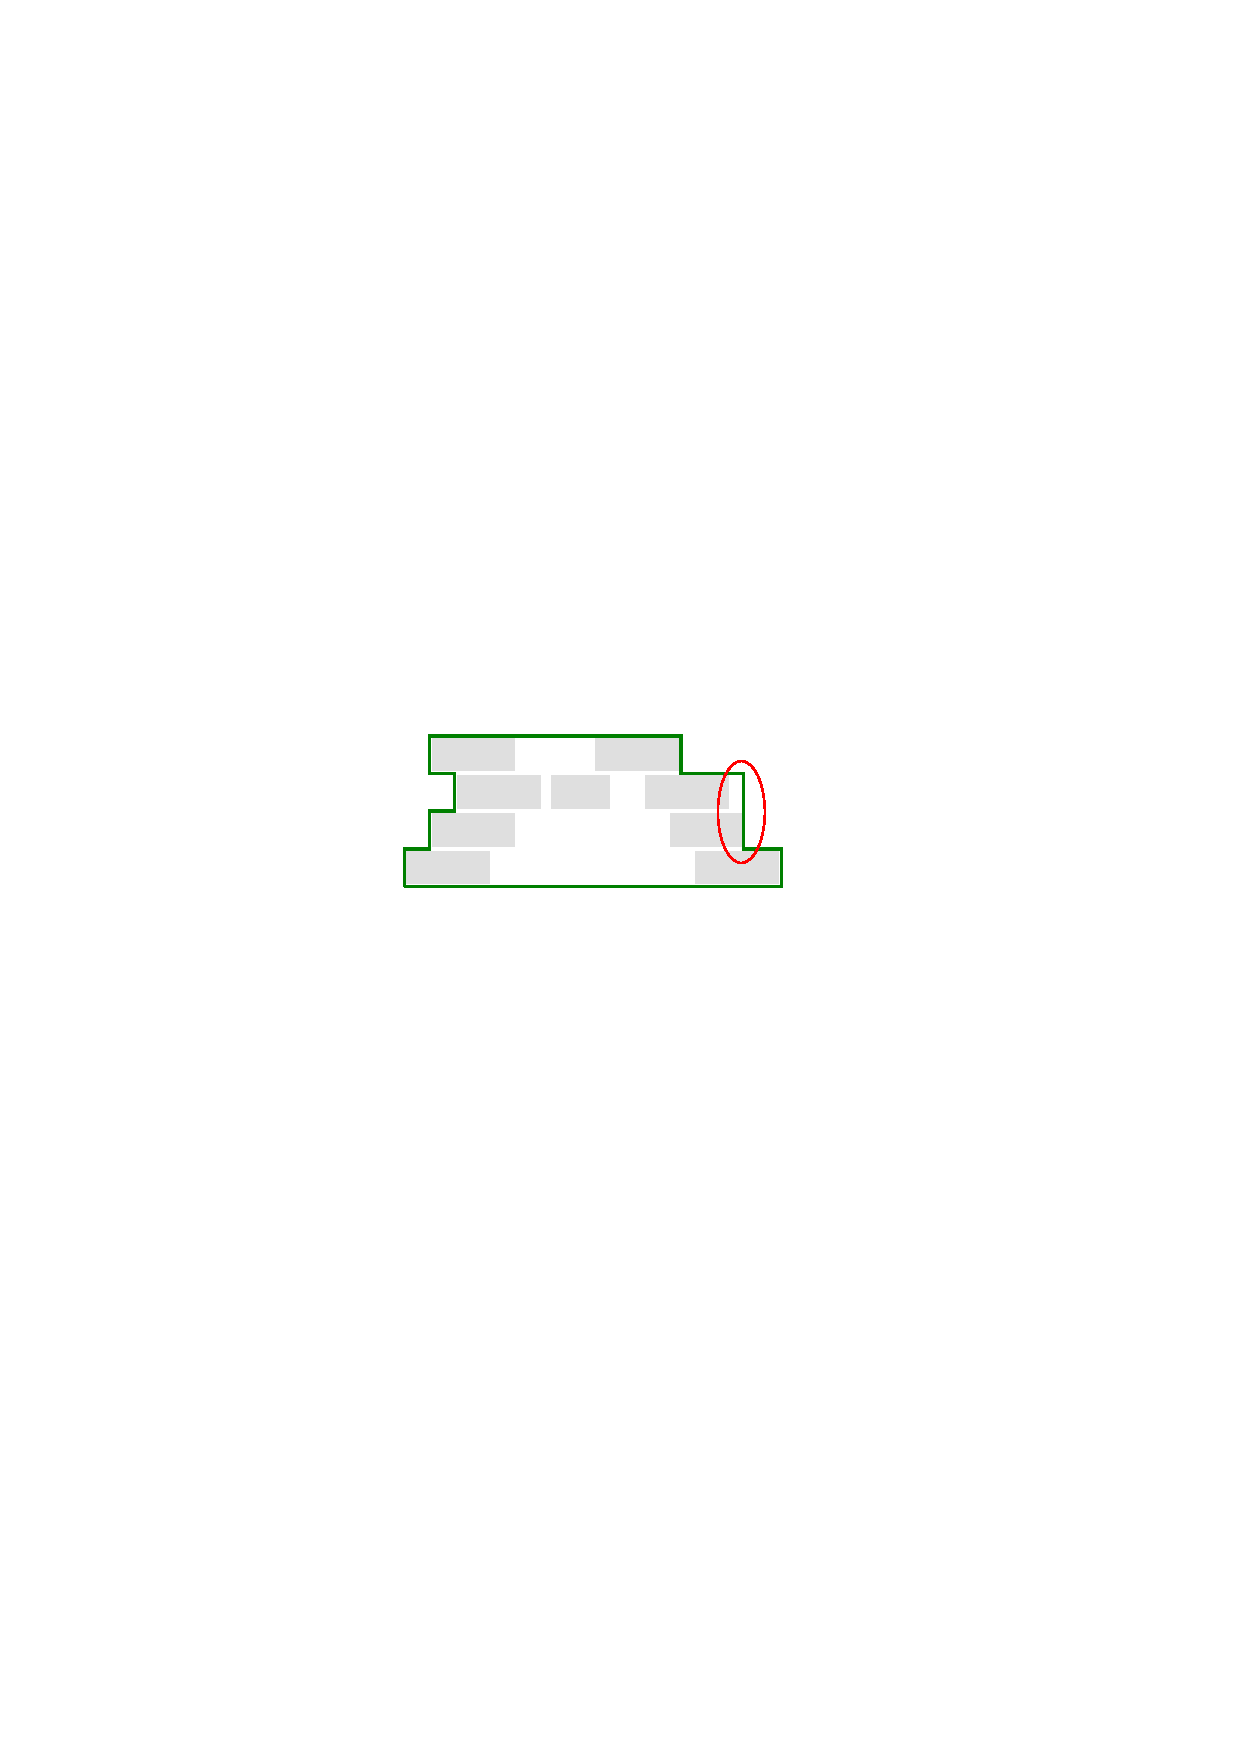
\includegraphics[width=.47\columnwidth]{figure5b}}
	\caption{Rectilinear shape generation.}
	\label{fig:shape}
\end{figure}

To reduce the number of line bends, the top and the bottom sides of the set outline are flattened. The left and right sides  are kept unchanged because they indicate the temporal information of events. On both sides, the outline can be ``jagged'' if two events start or end close to each other. Those close vertical segments are combined to reduce line bends if their horizontal gap is smaller than some threshold. This trades off time accuracy for outline smoothness and can be adjusted by the user. Figure~\ref{fig:shape2} shows the result of this simplification. 

To reduce the degree of line bends, vertical segments are converted to diagonal ones wherever possible, such as  $e_2$ and $e_3$ in Figure~\ref{fig:generation1}. Smoother lines are easier for users to follow~\cite{Kim2010}, thus diagonal segments are further converted to B\'{e}zier curves, and squared corners are replaced by quadrant arcs as in Figure~\ref{fig:generation2}.

\begin{figure}[ht]
	\centering
	\subcaptionbox{Vertical segments $e_2$ and $e_3$ are converted to diagonal ones (dashed lines).\label{fig:generation1}}
		{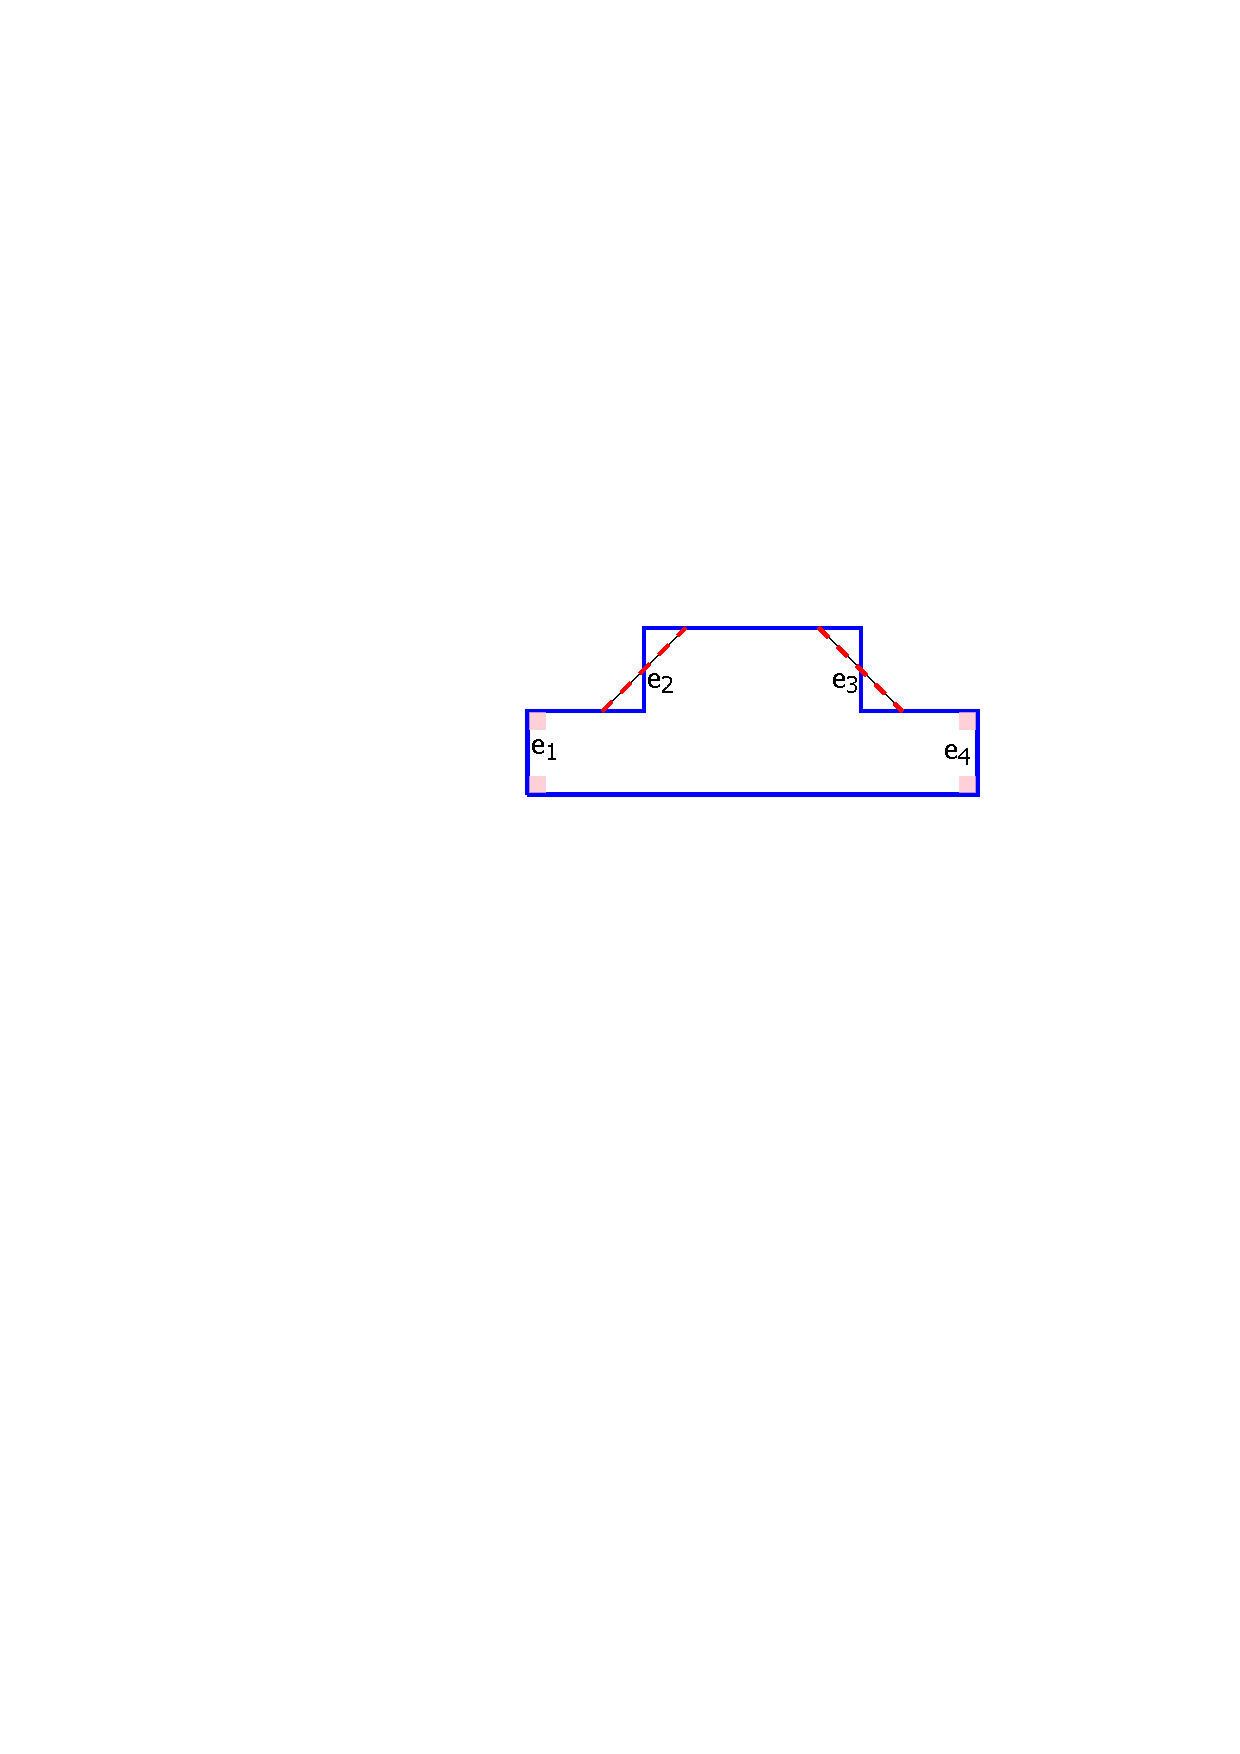
\includegraphics[width=.47\columnwidth]{figure6a}}
	\hfill
	\subcaptionbox{Squared corners are replaced by quadrant arcs. $e_2$ and $e_3$ are smoothened by B\'{e}zier curves.\label{fig:generation2}}
		{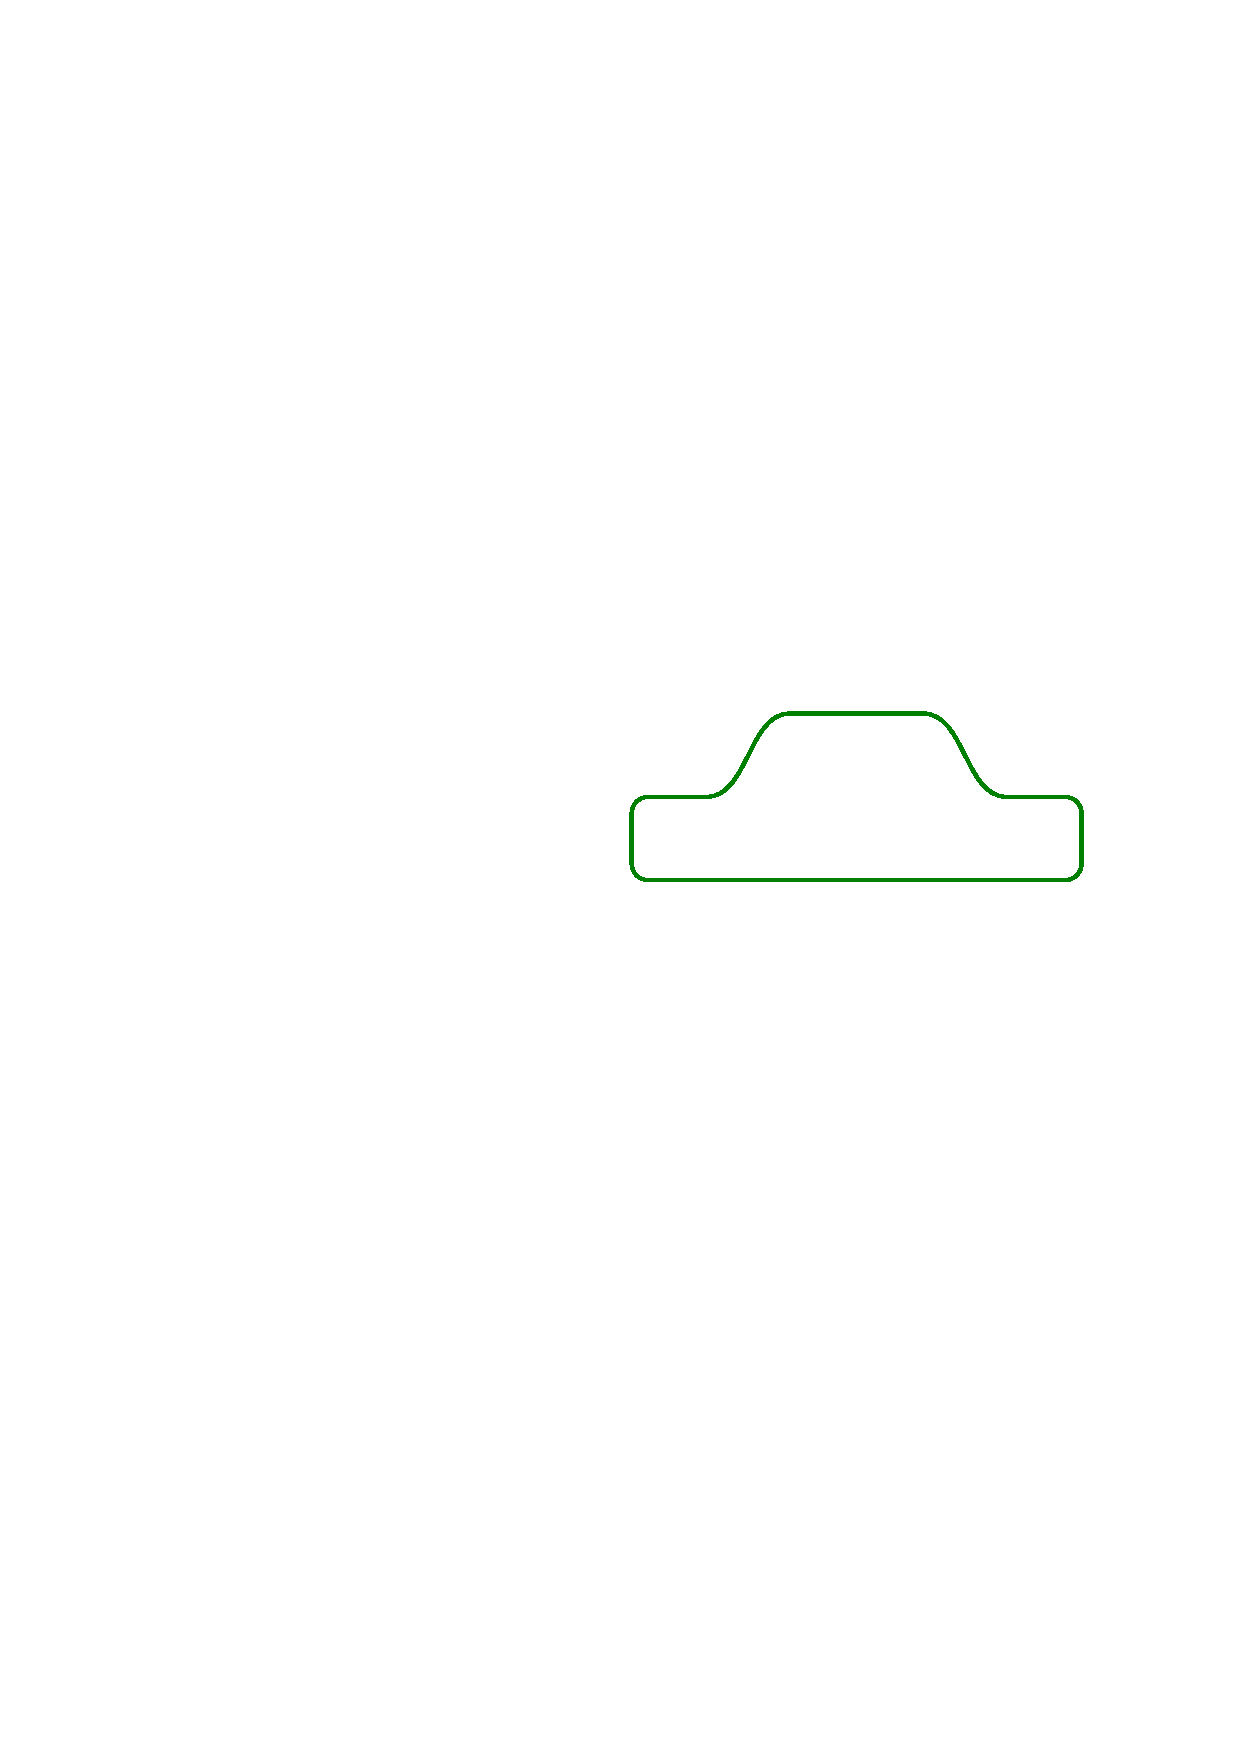
\includegraphics[width=.47\columnwidth]{figure6b}}
	\caption{Shape smoothening by reducing the degree of line bends.}
	\label{fig:generation}
\end{figure}

\subsubsection{Set Coloring}
Each set is filled with a color selected from Qualitative Set 2 of ColorBrewer~\cite{Harrower2003} to make them easily distinguishable. Two color filling options are considered: only the time circle and the entire label. Our design follows uniform connectedness principle requiring visual connection among same-set events. When they are visually connected and only their time circles are filled, intersection between edges and text may reduce the readability of the visualization. Figure~\ref{fig:evaluation2} shows an example of KelpFusion~\cite{Meulemans2013} using this approach. In the second option, filling the entire label may produce a false understanding about the temporal information of events. We choose this option and lessen the effect by coloring the gap between events as in Figure~\ref{fig:evaluation1}. It also helps increase the sense of grouping compared to filling only the time circles.

One common coloring method for set intersections is \emph{color blending} as used in Venn diagrams~\cite{Ware2013}. Color for each set is half-transparent, and alpha blending is applied to produce a new color for the intersection. However, the output color may look irrelevant to the two input colors and may be confused as the color for a new set rather than the intersection part.

To address this issue, we fill the intersection with a linear color gradient changing between the two set colors as in Figure~\ref{fig:gradient1}. While the gradient provides a smooth transition, it becomes difficult to recognize the two ends of the intersection. For example, it is not clear from Figure~\ref{fig:gradient1} that the background of the event ``Rove's 4th grand jury appearance'' (the second row from top to bottom) is pure yellow or it has a mix of green as well. To solve this problem, multiple color transitions are used instead of a single transition. For instance, in Figure~\ref{fig:gradient2}, the color transitions between green and yellow are repeated multiple times so that both colors are clearly shown in every row of the intersection.

\begin{figure}[!htb]
	\centering
	\subcaptionbox{Intersection as a single color gradient.\label{fig:gradient1}}
		{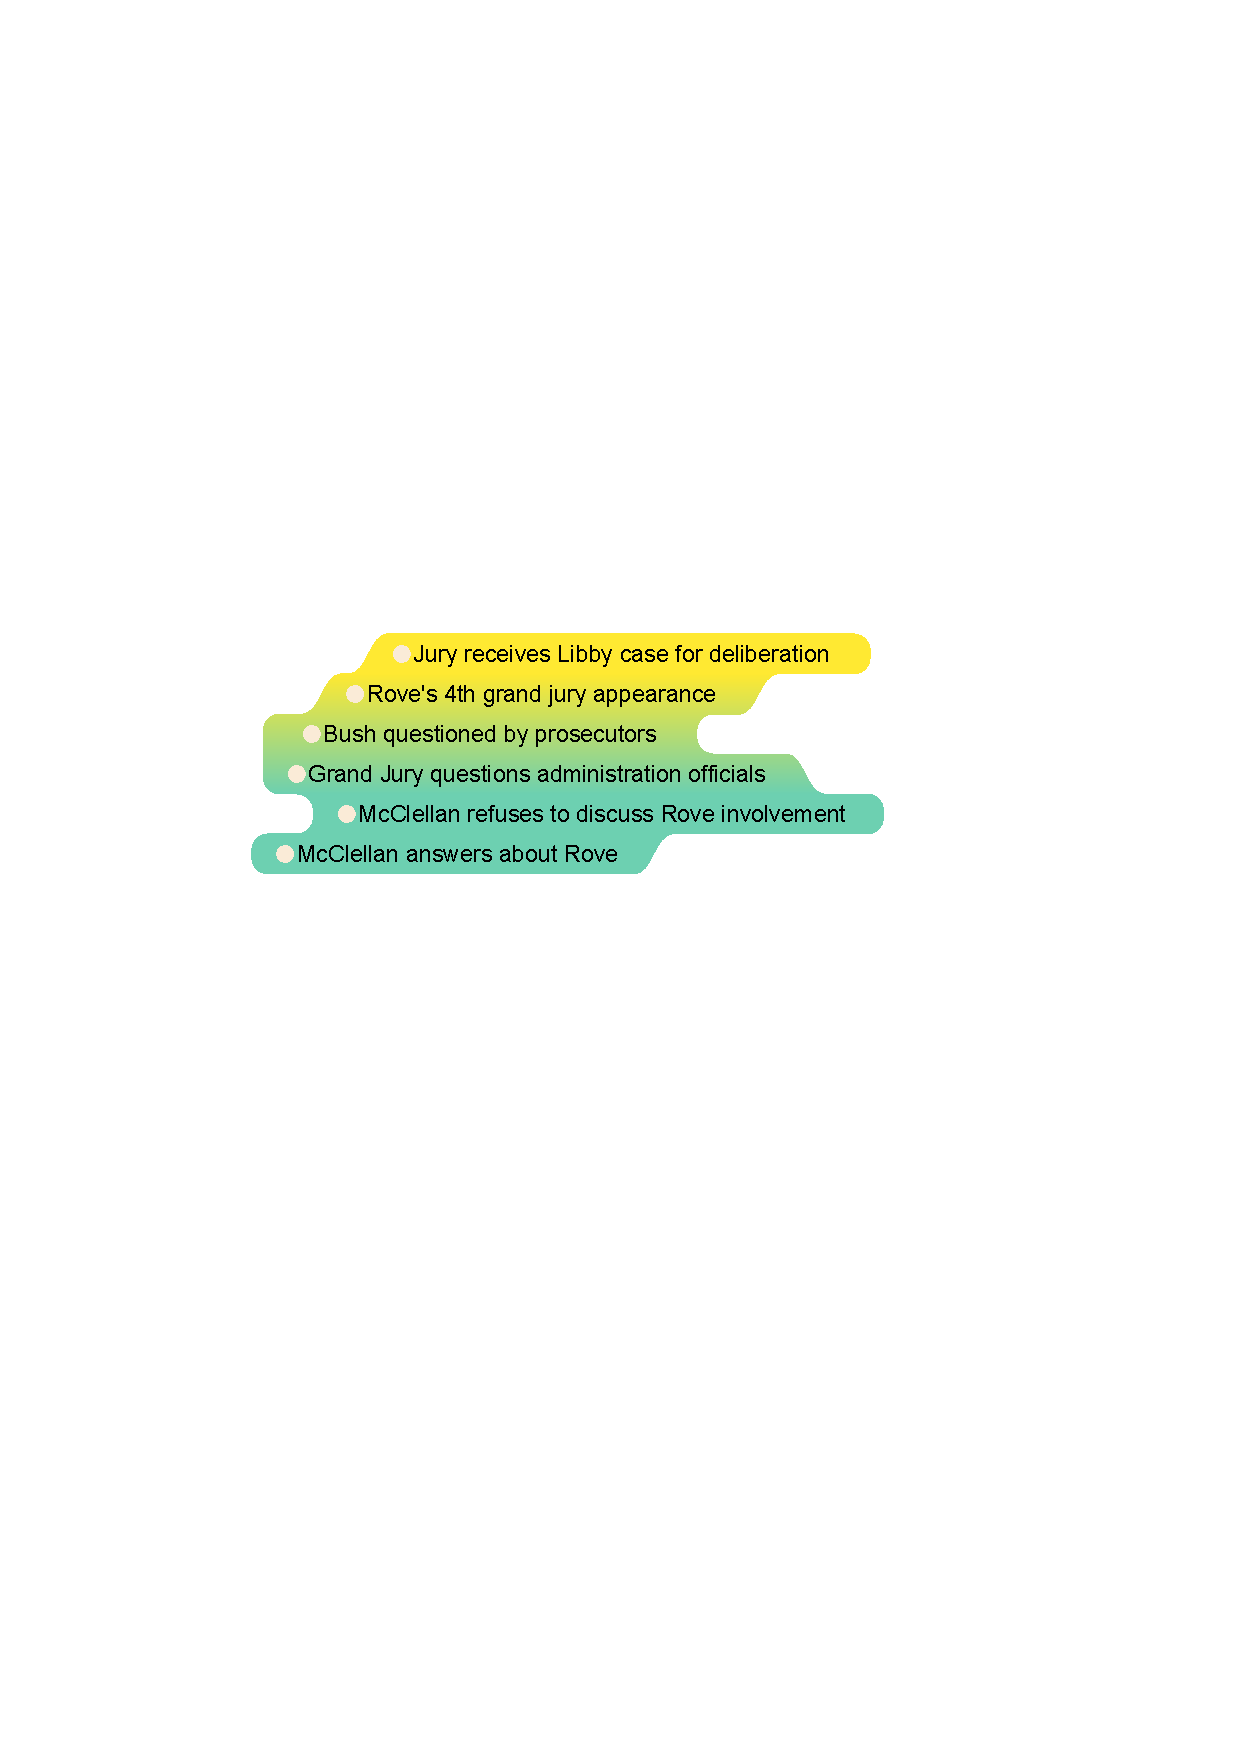
\includegraphics[width=0.47\columnwidth]{figure7a}}
	\hfill
	\subcaptionbox{Intersection as multiple color gradients.\label{fig:gradient2}}
		{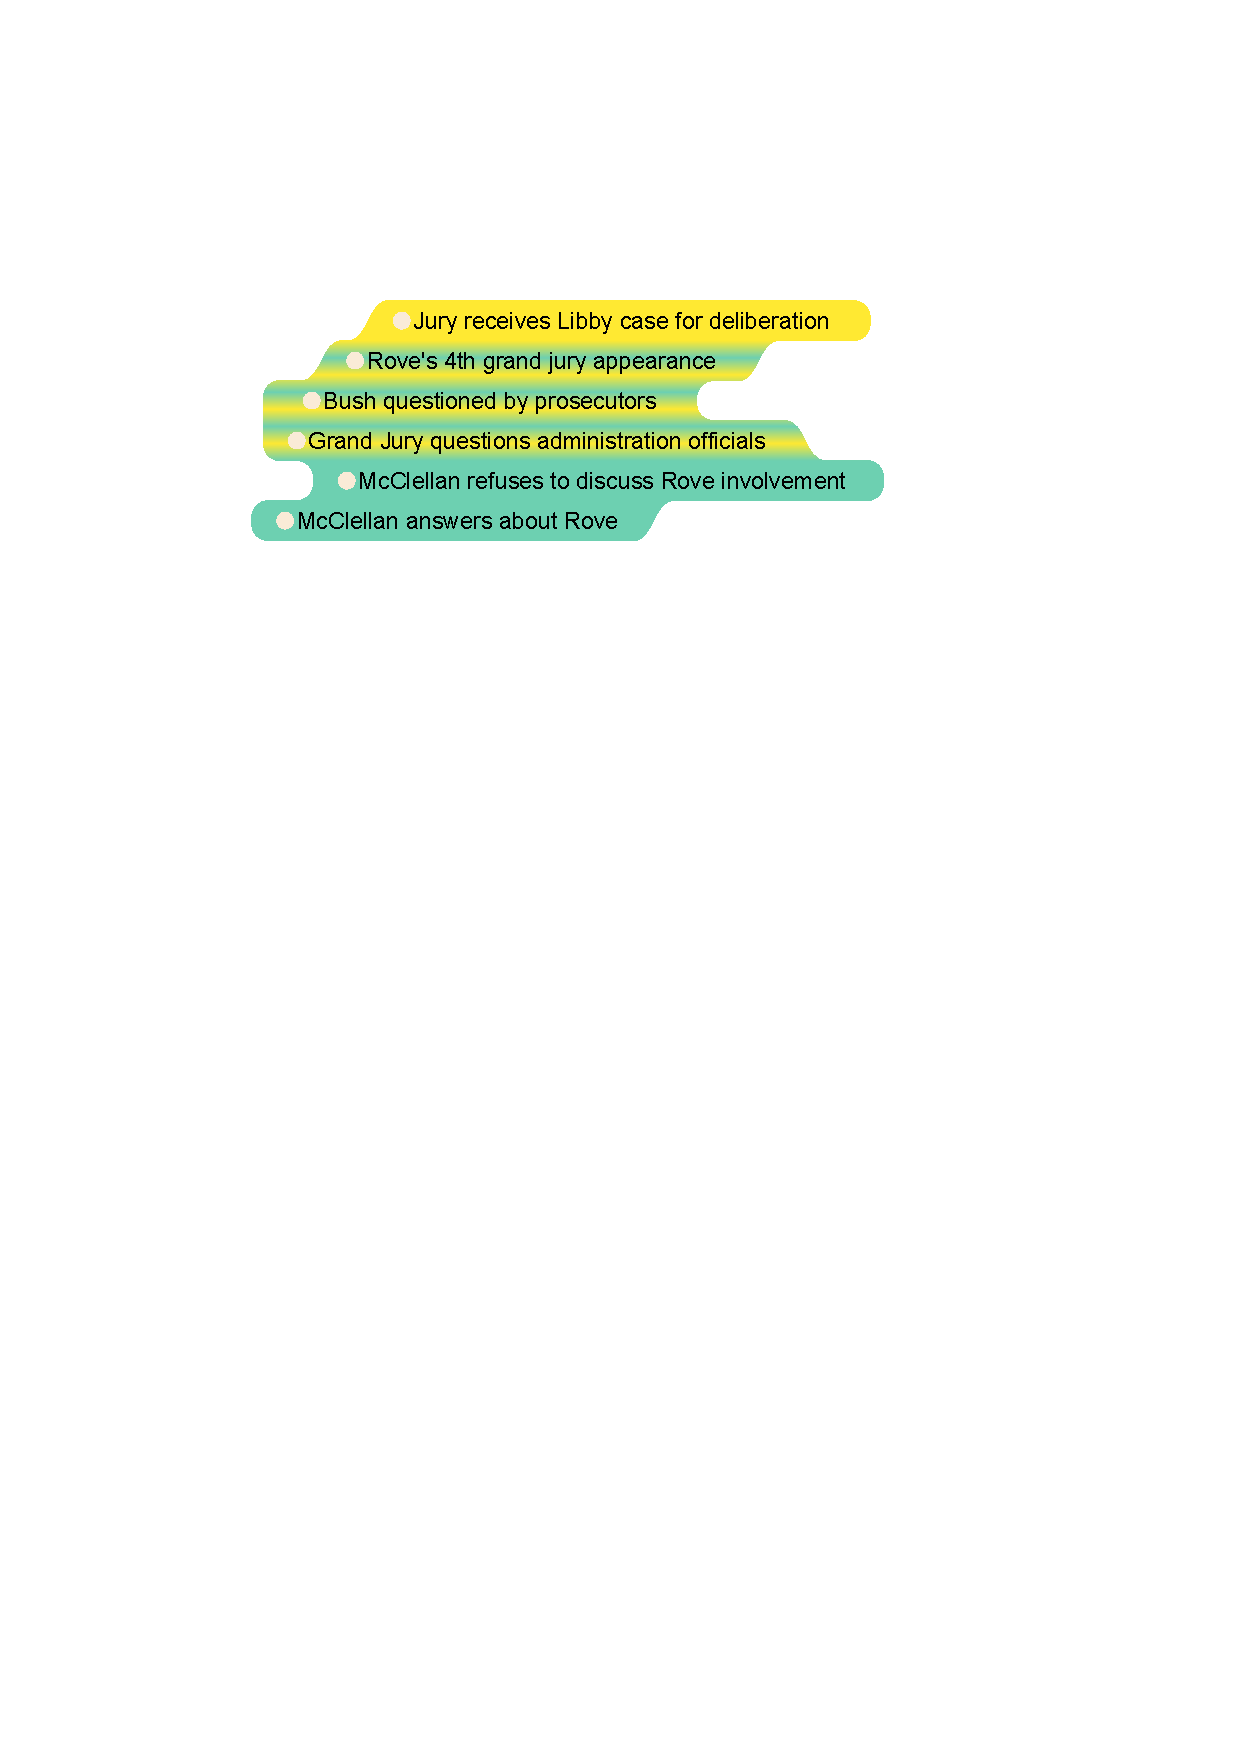
\includegraphics[width=0.47\columnwidth]{figure7b}}
	\caption{Visual representations of set intersections using color gradient.}
	\label{fig:gradient}
\end{figure}

\subsubsection{Multiple-set Events}
With the vertical layering of sets as discussed earlier, three sets cannot be placed adjacently; therefore, it is unable to visualize intersections among three sets or more. This is also a challenging problem with other state-of-the-art methods~\cite{Alsallakh2014}. To address this issue, similar to non-neighboring sets, we replicate events for each set that they belong to so that all events in the same set stay close together producing a compact visualization. To provide full set memberships of events, one method is connecting all replicates of the same event using edges. However, this may produce a cluttered visualization with many edge crossings. Another method is to color code the event according to its set memberships. The first option is to color the event time circle using either multiple circles (Figure~\ref{fig:eventmembership1}) or concentric rings (Figure~\ref{fig:eventmembership2}). The former requires more horizontal space, whereas the latter needs more vertical space. Another option is to color the background of the event label. Color gradient is used for a smooth color transition as in Figure~\ref{fig:eventmembership3}. This visual encoding is consistent with the use of color gradient to show two-set intersections. However, a timeline with many long-label events may produce a too colorful and distracted visualization. Also, limited label height may hamper the detection of color transition. To solve these problems, color is transitioned from left to right, and only run through a first few characters of the event label (Figure~\ref{fig:eventmembership4}). Figure~\ref{fig:citations} shows this technique in a visualization of 200 events.

\begin{figure}[!htb]
	\centering
	\subcaptionbox{Circles represent sets.\label{fig:eventmembership1}}[.22\columnwidth]{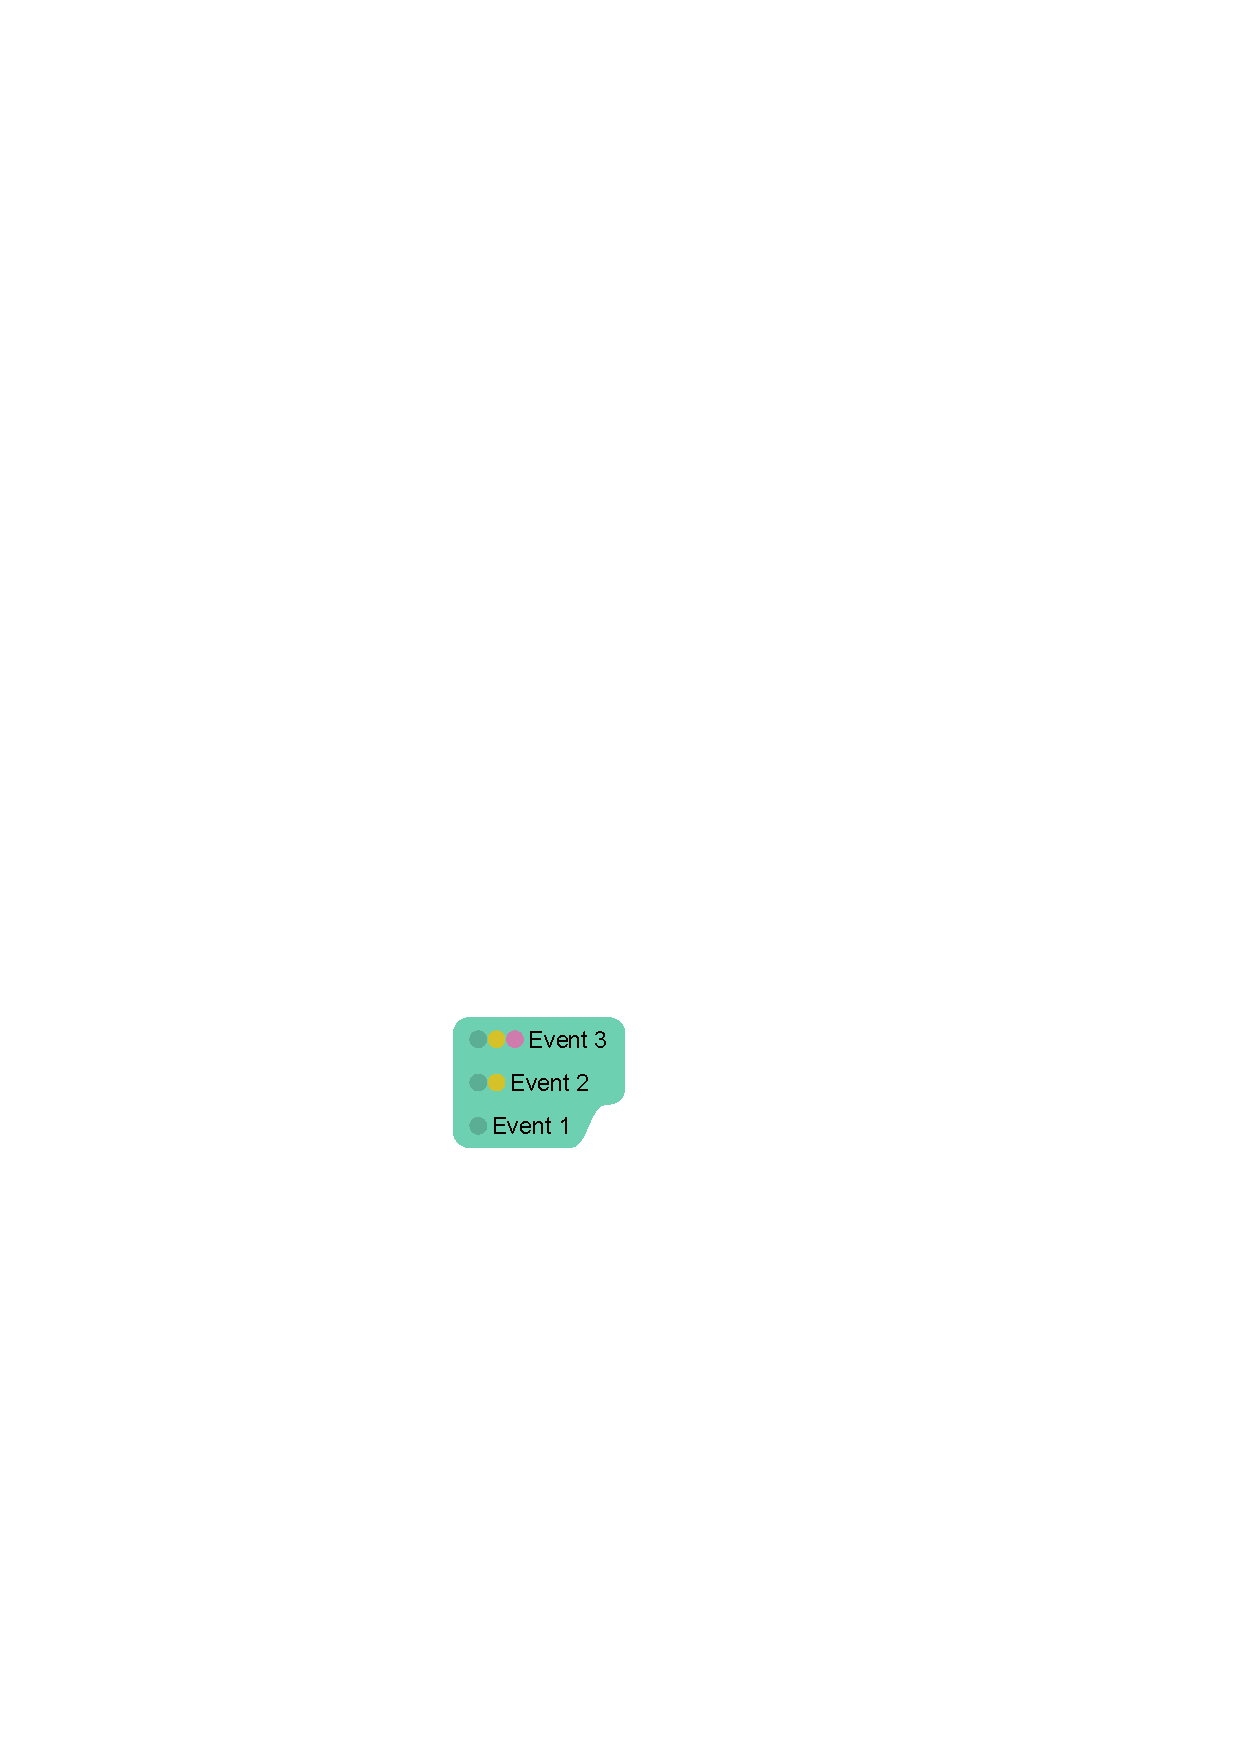
\includegraphics[height=.15\columnwidth]{figure8a}}
	\hfill
	\subcaptionbox{Rings represent sets.\label{fig:eventmembership2}}[.22\columnwidth]{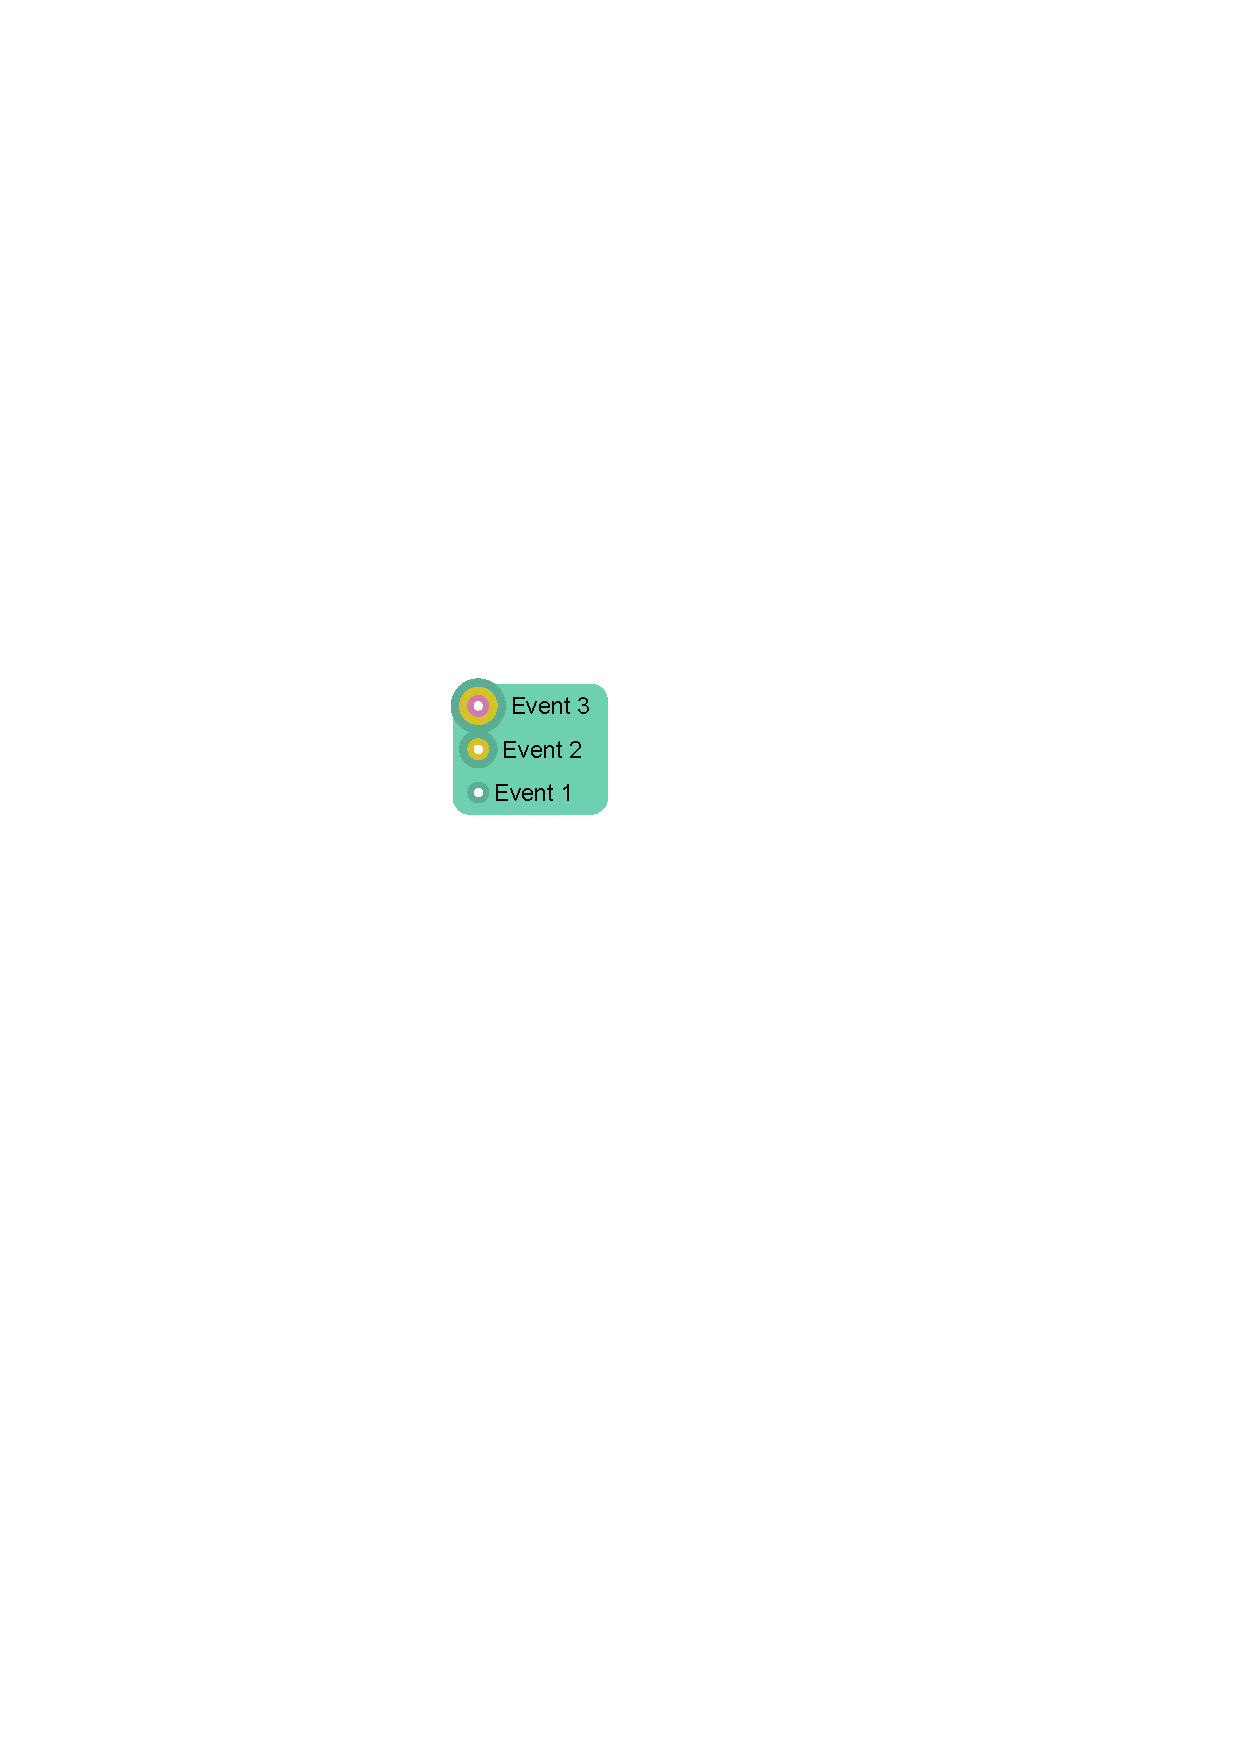
\includegraphics[height=.156\columnwidth]{figure8b}}
	\hfill
	\subcaptionbox{Vertical gradients represent sets.\label{fig:eventmembership3}}[.22\columnwidth]{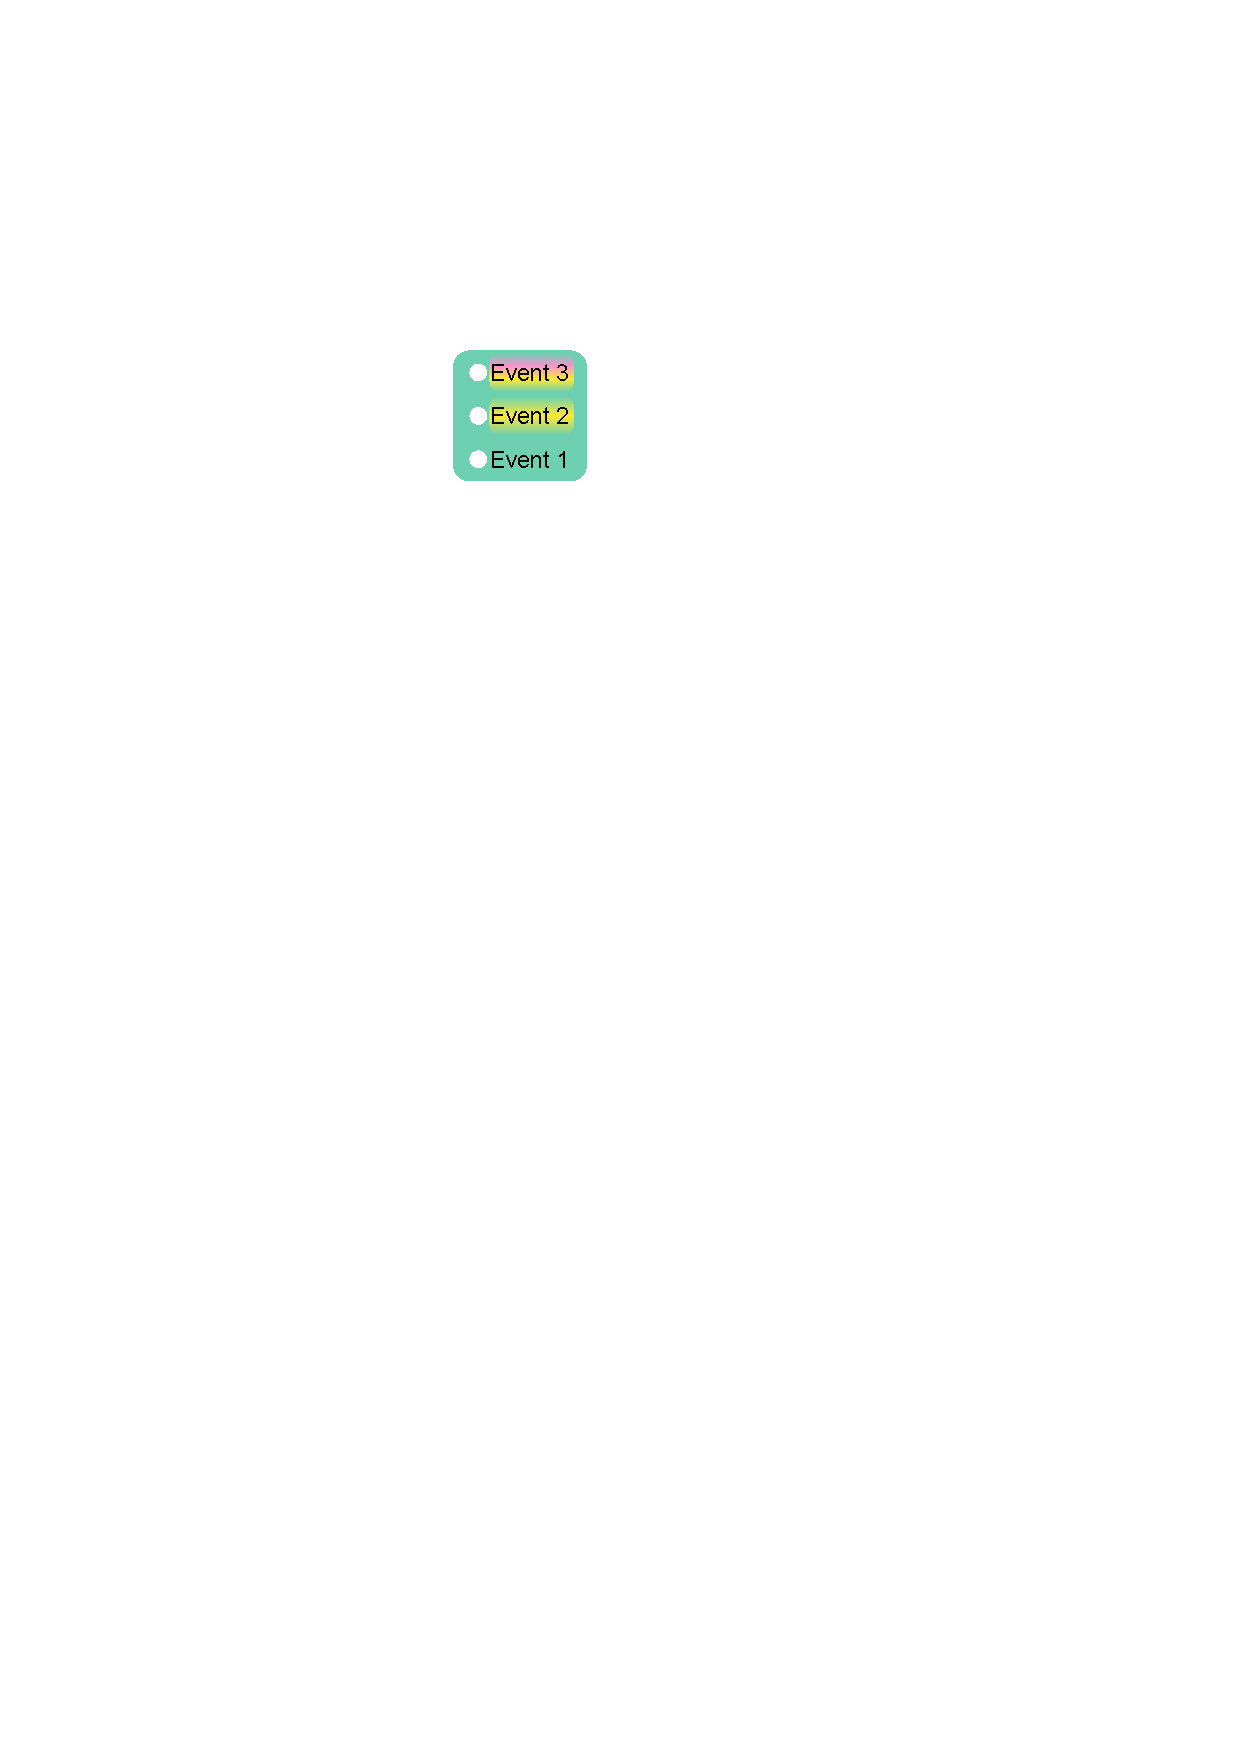
\includegraphics[height=.15\columnwidth]{figure8c}}
	\hfill
	\subcaptionbox{Horizontal gradients represent sets.\label{fig:eventmembership4}}[.22\columnwidth]{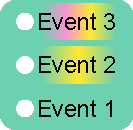
\includegraphics[height=.15\columnwidth]{figure8d}}
	\caption{Visual representations of multiple-set events. Event 1 is single-set (green). Event 2 is double-set (green, yellow). Event 3 is triple-set (green, yellow, pink).}
	\label{fig:eventmembership}
\end{figure}

For interval events, only coloring the background of labels can be used because they do not have time circles, which can be added but at the cost of extra display space. Time bars can be used to show set memberships by dividing into multiple horizontal parts, each color for one set. However, this could be misinterpreted as an event having different set membership in each part of its timespan.

Putting it all together, Figure~\ref{fig:ts-overview} shows a TimeSets visualization with the CIA leak case dataset~\footnote{\url{http://www.npr.org/templates/story/story.php?storyId=4764919}}, in which the identity of CIA operative Valerie Plame was made public. The algorithm to produce this visualization is described in Section~\ref{sec:ts-algorithm}.

\begin{figure}[!htb]
	\centering
	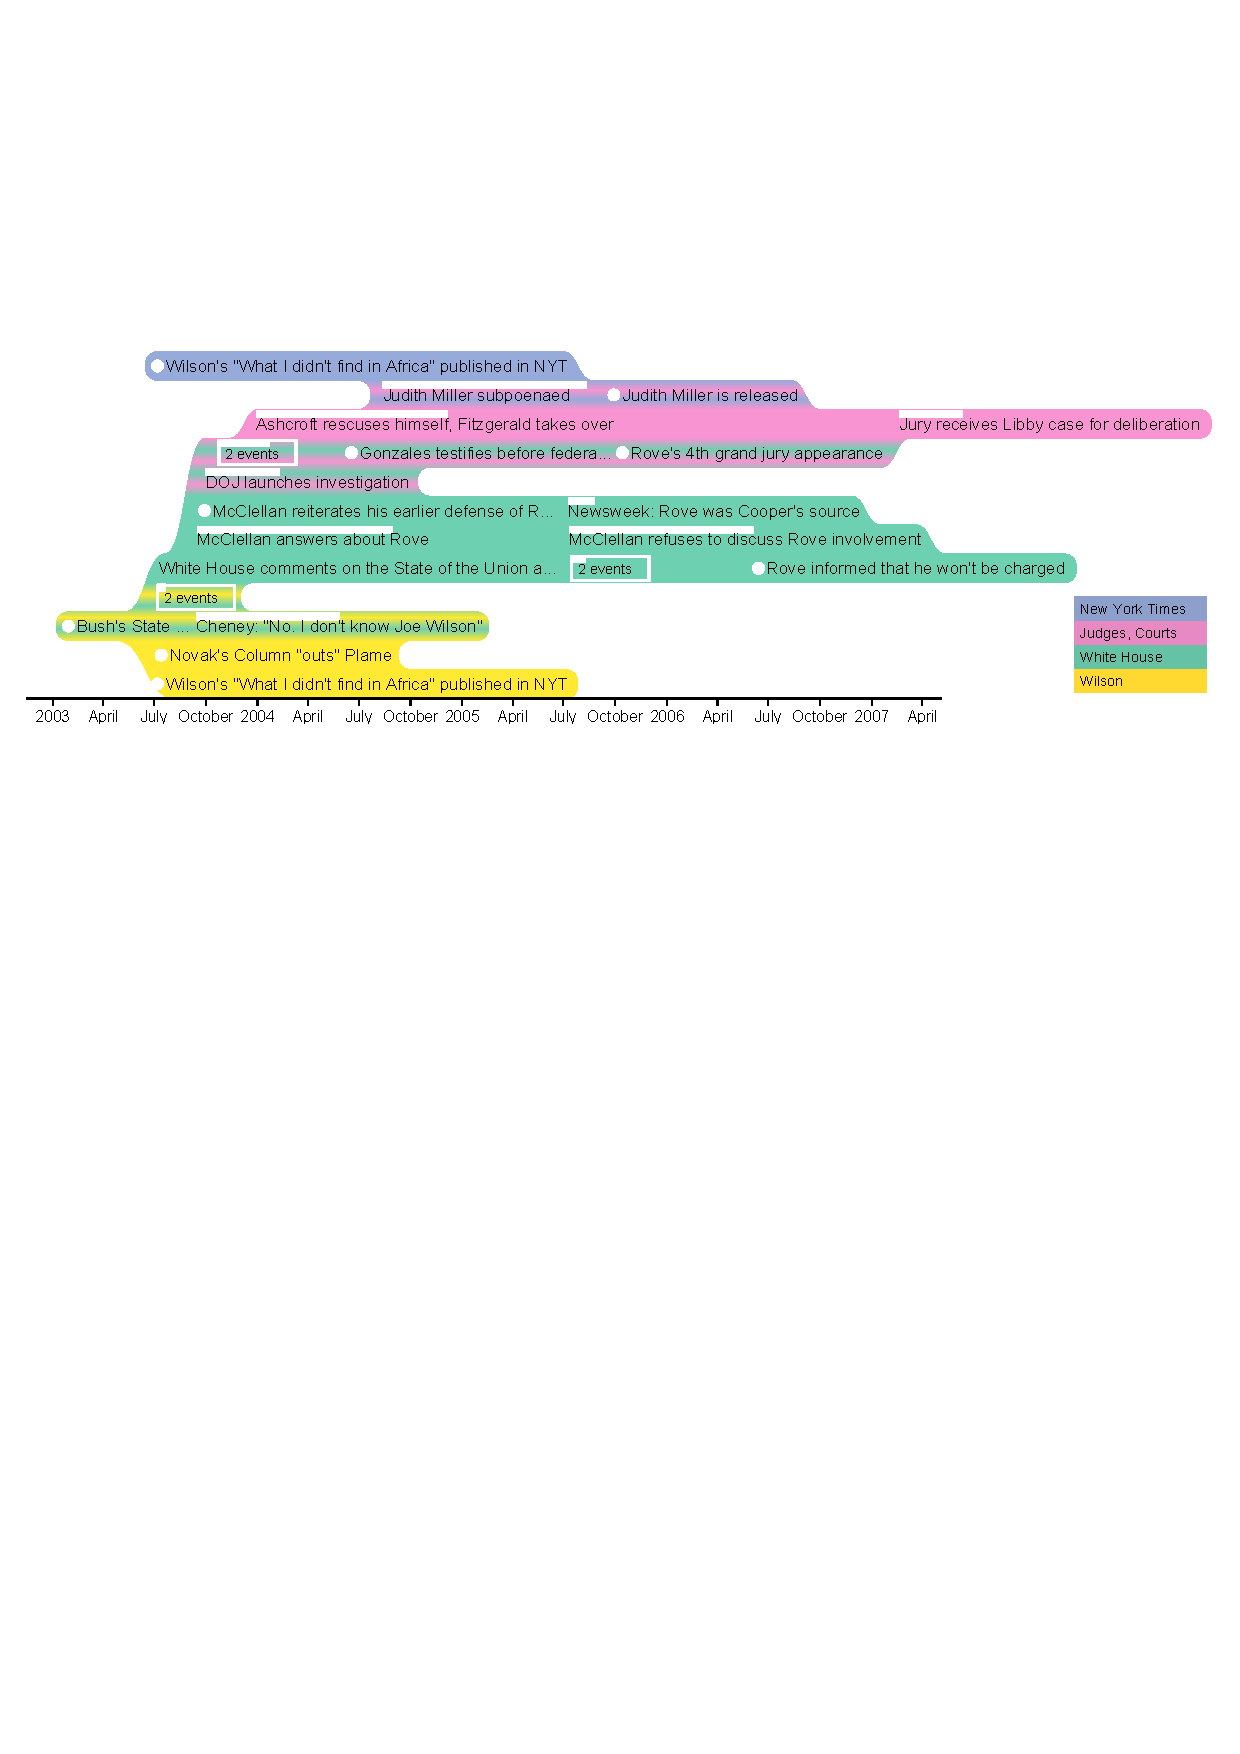
\includegraphics[width=\linewidth]{figure1}
	\caption{TimeSets visualization of the CIA leak case. The timeline contains events that happened from 2002 to 2007, each includes a timestamp, a label, and topics such as ``White House''. Events are positioned along the horizontal time axis based on their temporal values, and vertically grouped by colored topics (see the color legend in the bottom right corner).}
	\label{fig:ts-overview}
\end{figure}

\subsection{Interaction}
\label{sub:interaction}
Interactive features are implemented to support timeline exploration. Mouse hovering an event reveals its temporal information and the complete label. When none of the multiple-set visualization techniques proposed earlier is used to statically display the full set memberships of an event, it is possible to use interaction to reveal that information. When an event is hovered, all of its replicates are highlighted, allowing easy examination of its full set memberships. This method prevents adding extra ink to the visualization; however, it requires users to discover the set information manually. 

TimeSets provides interactive set filtering and focused time window changing via zooming and panning. Clicking on a set in the legend (bottom-right corner in Figure~\ref{fig:ts-overview}) toggles its visibility. Time zoom is performed via the mouse-wheel button and pan is controlled by dragging the left mouse button. Users can also interactively modify set ordering by changing the order in the legend through drag-and-drop. A smooth animated transition is provided for all the interactions to help users maintain their mental maps~\cite{Elmqvist2011}.